\documentclass[11pt]{article}
\usepackage[utf8]{inputenc}
\usepackage[T1]{fontenc}
\usepackage[spanish,es-noshorthands]{babel}
\usepackage[margin=2.5cm]{geometry}
\usepackage{amsmath,amssymb}
\usepackage{graphicx}
\usepackage{booktabs}
\usepackage{xcolor}
\usepackage[colorlinks=true,linkcolor=blue,citecolor=blue,urlcolor=blue]{hyperref}
\usepackage{caption}
\usepackage{parskip}
\usepackage[expansion=false]{microtype}
\sloppy

\title{\textbf{Una fórmula barata para el $\beta$ óptimo\\ de una crossbar memristiva}\\
\large Síntesis del proyecto: de la idea original a un reemplazo validado del grid-search}
\author{Walter Quiñonez}
\date{Trabajo realizado con Claude Code \textperiodcentered\ Proyecto final del curso}

\begin{document}
\maketitle

\begin{quote}\itshape
El softmax de una crossbar memristiva es $\mathrm{softmax}(\beta\cdot I)$, y elegir $\beta$
por grid-search+K-fold es caro. Este proyecto encuentra una fórmula de dos factores
($\sigma_W$, dispersión de pesos; $\mathrm{paso\_medio}$, granularidad de la curva
potenciación/depresión) que predice el $\beta$ óptimo \textbf{antes de entrenar}, la valida
contra 30 grid-searches reales completos ($R^2=0.930$), y la usa para reemplazar la grilla
ciega de \texttt{search\_best\_beta()} por una búsqueda angosta centrada en la predicción
—bajando el \emph{regret} medido de 10.19 puntos porcentuales a 0.08.
\end{quote}

\tableofcontents

\section{El problema}

En una red neuronal implementada sobre una crossbar memristiva, cada corriente de salida
$I_i = \sum_j (G^+_{ij}-G^-_{ij})\,V_j$ pasa por una no linealidad $O_i=f(\beta\cdot I_i)$
(softmax o tanh, según la capa). El valor de $\beta$ determina si esa no linealidad satura o
queda demasiado chata, y el accuracy final depende fuertemente de él. El único método
disponible en el código base para elegirlo, \texttt{search\_best\_beta()}, es un grid-search
con K-fold: cientos de entrenamientos cortos por cada $\beta$ candidato. La pregunta de este
proyecto: ¿se puede estimar un $\beta$ cercano al óptimo sin entrenar nada, usando solo
propiedades de la curva de potenciación/depresión (P/D) del dispositivo memristivo?

\section{Punto de partida teórico}

\texttt{papers/Reporte\_beta\_optimo\_analitico.pdf} (reporte previo del proyecto) deriva una
fórmula candidata modelando la corriente como una suma de $N$ términos aproximadamente
independientes (Teorema Central del Límite), siguiendo el mismo esquema
$I=\sum_j W_{ij}V_j$, $f=\tanh(\beta I)$ que Prezioso et al. (\emph{Nature} 521, 61, 2015)
atribuyen a la recomendación de LeCun et al. (\emph{Efficient Backprop}, 1998):
$$\sigma_I = \sqrt{N}\cdot\sigma_W\cdot V_{rms} \qquad\Rightarrow\qquad
\beta_{\text{óptimo}} \approx \frac{\kappa}{\sqrt{N}\,\sigma_W\,V_{rms}}$$
con $\sigma_W$ el desvío estándar de los pesos $W=G^+-G^-$ bajo la inicialización aleatoria
del código, $V_{rms}=\sqrt{E[V^2]}$ de los voltajes de entrada (píxeles de MNIST), y $\kappa$
una constante $O(1\text{--}10)$.

\section{Idea original y sus sesgos}

\texttt{analisis\_beta\_optimo.py} (raíz del repo) fue el primer intento de poner a prueba
esta idea con un Monte Carlo de pesos y corrientes. \texttt{analisis\_corrientes\_beta\_optimo/}
encontró que ese script tenía dos sesgos que rompían la premisa $E[I]\approx0$ que asume la
fórmula: armaba los pesos como una matriz combinatoria $pot_i-dep_j$ en vez de sortear
$G^+$ y $G^-$ independientemente (como hace la red real vía \texttt{G0\_initialization}), y
muestreaba los voltajes de los valores únicos de píxel en vez de respetar que el 81\,\% de los
píxeles reales de MNIST son exactamente 0.

\begin{figure}[h]\centering
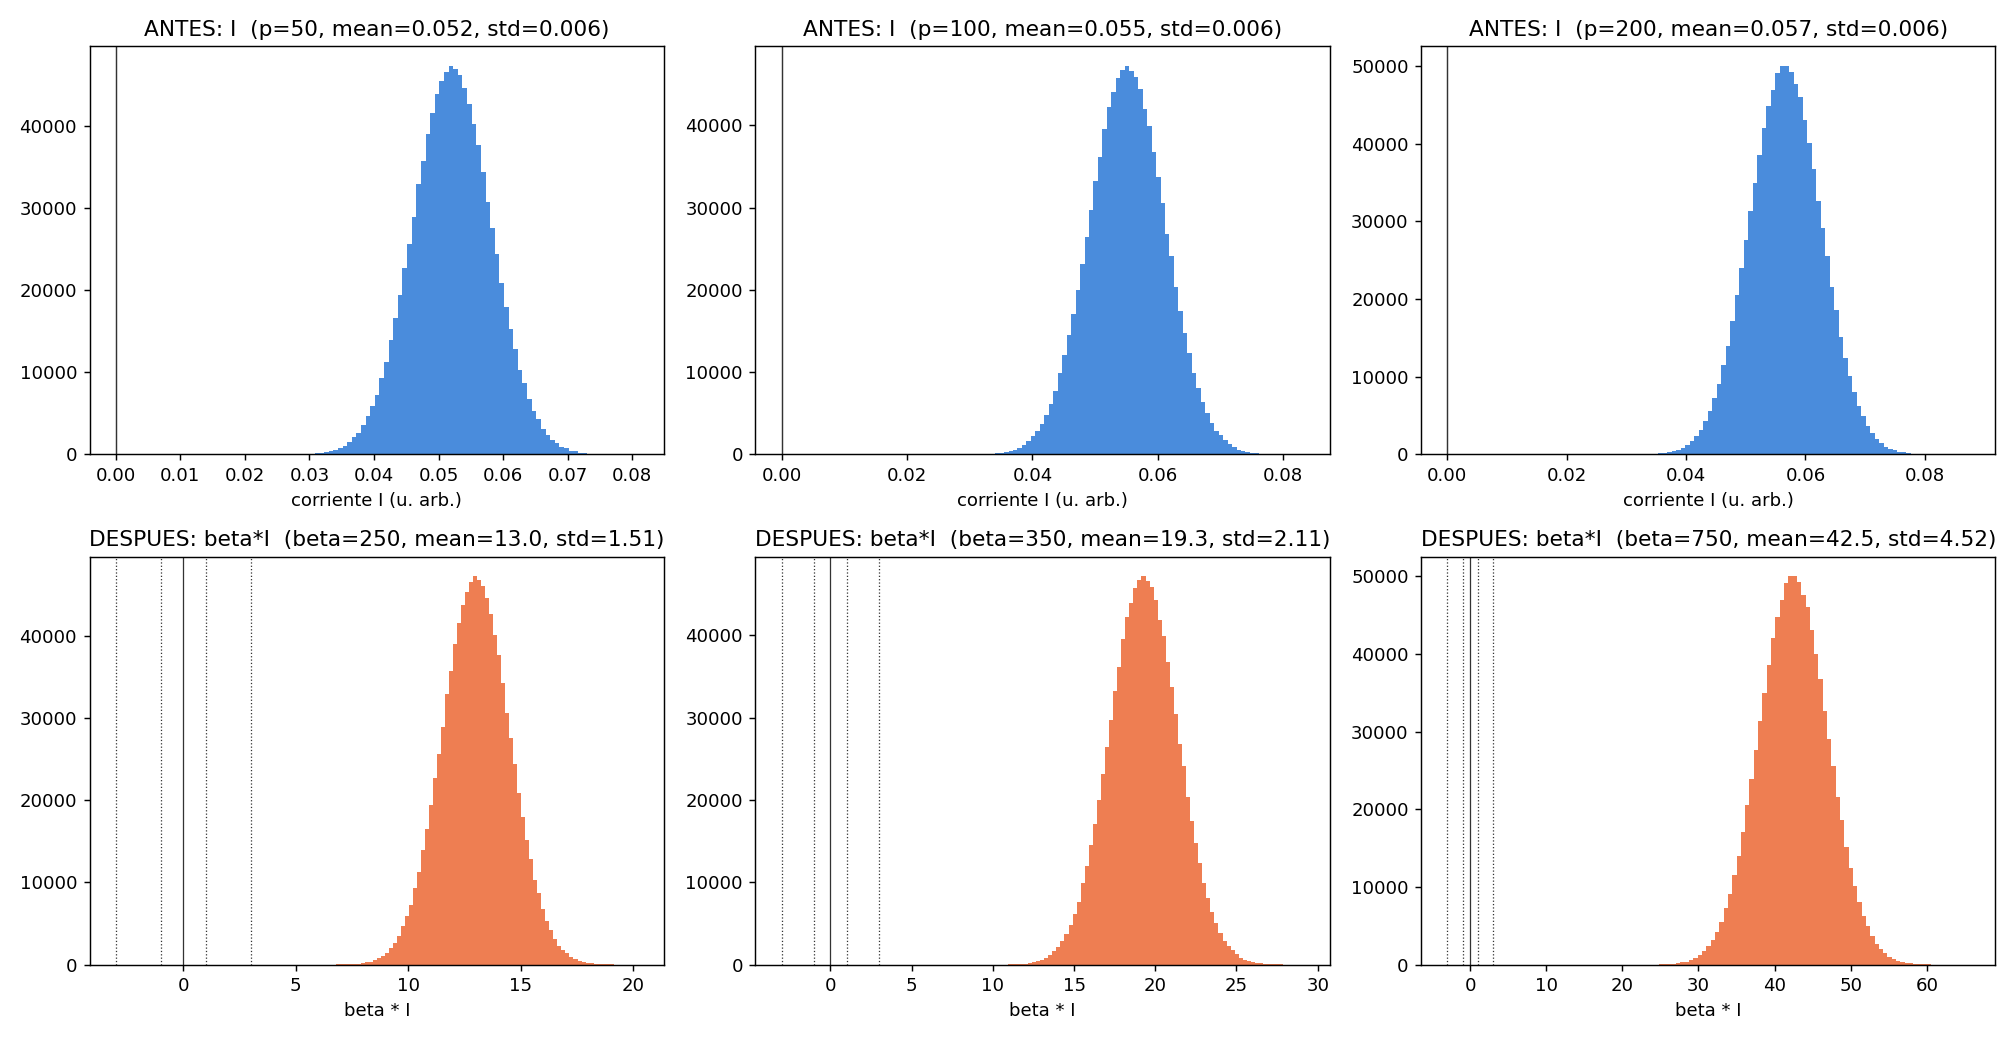
\includegraphics[width=.7\linewidth]{../analisis_corrientes_beta_optimo/corrientes_antes_despues_beta.png}
\caption{Distribución de corriente Monte Carlo antes y después de corregir los dos sesgos identificados.}
\end{figure}

\section{Primera validación (6 curvas reales)}

\texttt{validacion\_formula\_beta\_optimo/} puso la fórmula ($\kappa=1$) a prueba contra
\textbf{6 grid-searches reales completos} (100 épocas, 20 series, 5 folds cada uno) —no una
búsqueda reducida. Resultado: \textbf{acierta el orden de magnitud} ($\kappa$ implicado
$\approx0.97$, dentro de $O(1\text{--}10)$) y \textbf{la dirección entre ventanas de
conductancia distintas} ($\sigma_W$ más grande $\Rightarrow$ $\beta$ óptimo más chico), pero
\textbf{no explica} la dependencia con el número de pulsos $p$ de la curva P/D a INL nominal
fijo: $\beta$ óptimo sube claramente con $p$ mientras $\sigma_W$ se mantiene casi constante
por diseño del experimento.

\begin{figure}[h]\centering
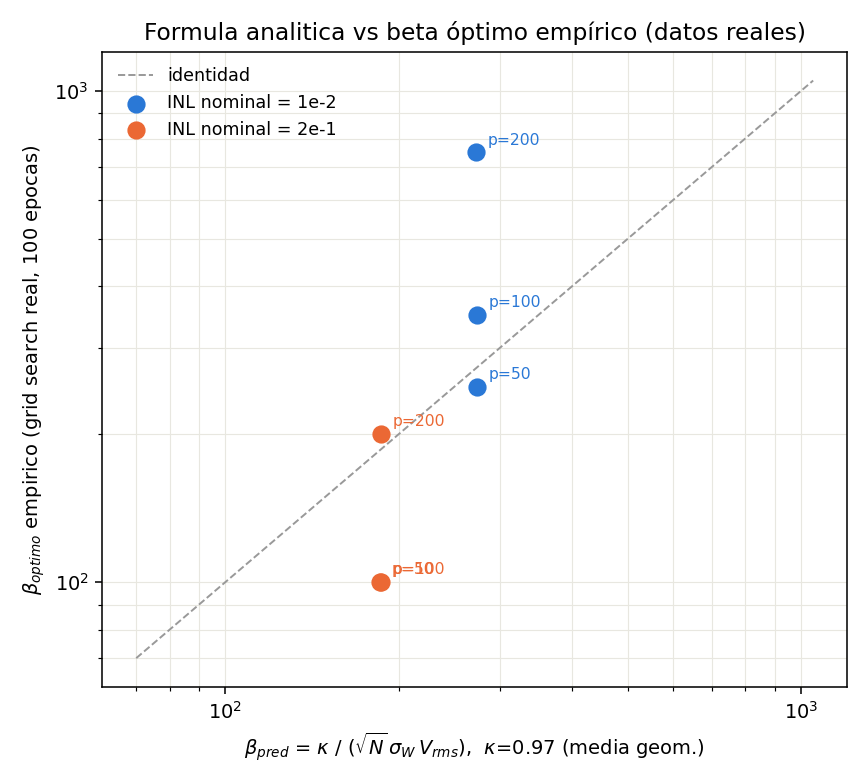
\includegraphics[width=.48\linewidth]{../validacion_formula_beta_optimo/beta_pred_vs_empirico.png}
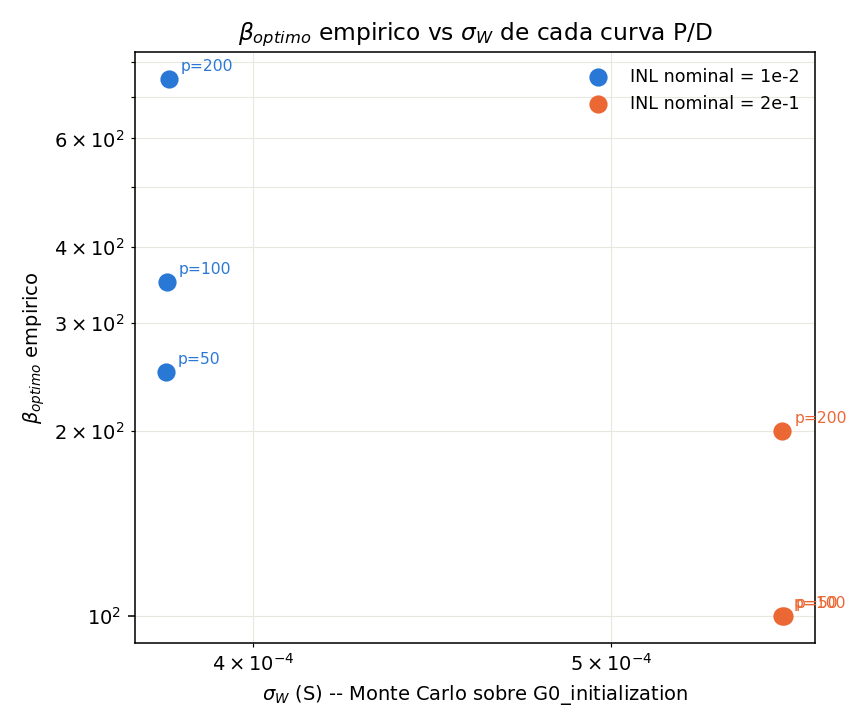
\includegraphics[width=.48\linewidth]{../validacion_formula_beta_optimo/beta_pred_vs_sigmaW.png}
\caption{Izq.: $\beta$ predicho ($\kappa=1$) vs. empírico. Der.: $\beta$ óptimo vs. $\sigma_W$
—acierta la dirección entre grupos de INL, no dentro de un grupo.}
\end{figure}

\section{La fórmula combinada}

\texttt{formula\_beta\_optimo\_propuesta/} combina $\sigma_W$ (predice la dirección entre
ventanas de conductancia) con el \textbf{paso medio} de la curva de potenciación,
$\mathrm{mean}(|pot_{i+1}-pot_i|)$ (predice la dirección con $p$), usando el Monte Carlo ya
corregido:
$$\beta_{\text{óptimo}} \approx 1.12\times10^{-11}\cdot\sigma_W^{-3.02}\cdot\mathrm{paso\_medio}^{-0.64}$$

\begin{table}[h]\centering
\begin{tabular}{lr}\toprule
Modelo & $R^2$ \\\midrule
solo $\sigma_W$ & 0.678 \\
solo $\mathrm{paso\_medio}$ & 0.273 \\
\textbf{combinado} & \textbf{0.947} \\\bottomrule
\end{tabular}
\caption{Regresión log-log sobre los mismos 6 puntos de la Sección 4.}
\end{table}

\begin{figure}[h]\centering
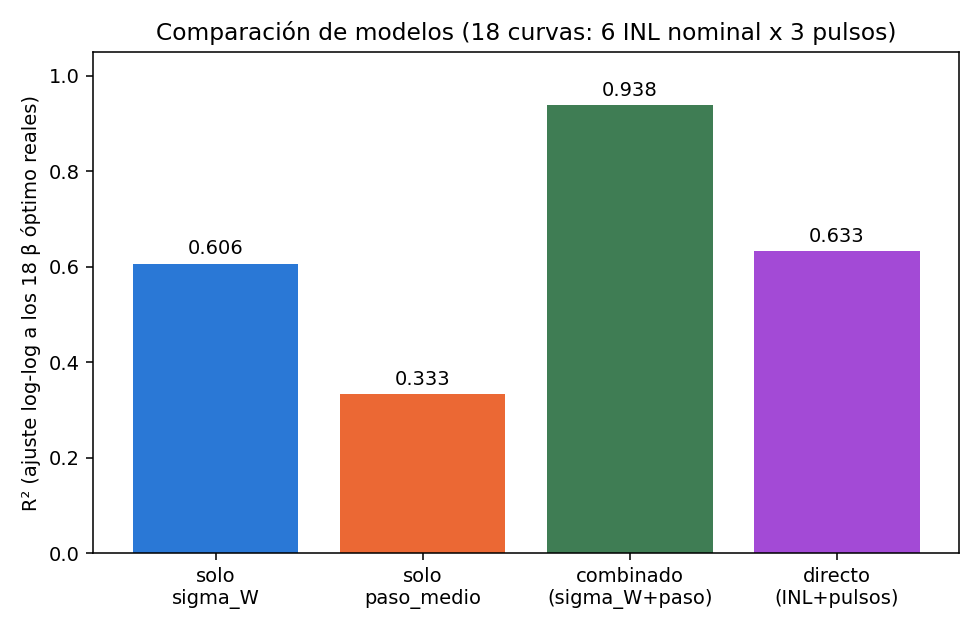
\includegraphics[width=.48\linewidth]{../formula_beta_optimo_propuesta/comparacion_R2_v2.png}
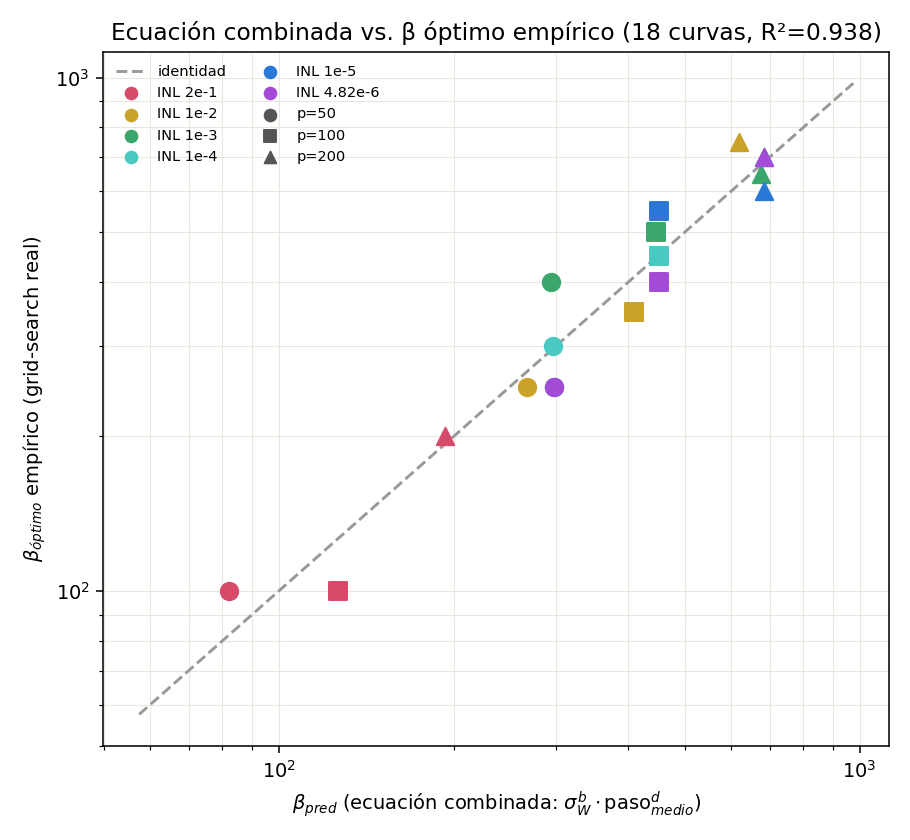
\includegraphics[width=.48\linewidth]{../formula_beta_optimo_propuesta/beta_pred_combinada_vs_empirico_v2.png}
\caption{Izq.: $R^2$ de cada modelo. Der.: $\beta$ predicho por la ecuación combinada vs. empírico.}
\end{figure}

\section{Reconfirmación a escala (18 $\to$ 30 curvas)}

\texttt{reconstruccion\_beta\_optimo\_18curvas/} y luego
\texttt{reconstruccion\_beta\_optimo\_30curvas/} repiten el mismo método (sin reentrenar nada
—Monte Carlo barato + reconstrucción determinista de logits ya guardados) sobre 18 y luego 30
curvas P/D reales (10 valores de INL nominal $\times$ 3 recuentos de pulsos). Los coeficientes
se mantienen prácticamente idénticos al triplicar-y-medio la muestra:

\begin{table}[h]\centering
\begin{tabular}{lrrr}\toprule
 & 6 curvas & 18 curvas & 30 curvas \\\midrule
exponente de $\sigma_I$ & $-3.02$ & $-3.06$ & $-3.00$ \\
exponente de $\mathrm{paso\_medio}$ & $-0.64$ & $-0.61$ & $-0.62$ \\
$R^2$ (log-log) & 0.947 & 0.938 & 0.930 \\\bottomrule
\end{tabular}
\end{table}

\begin{figure}[h]\centering
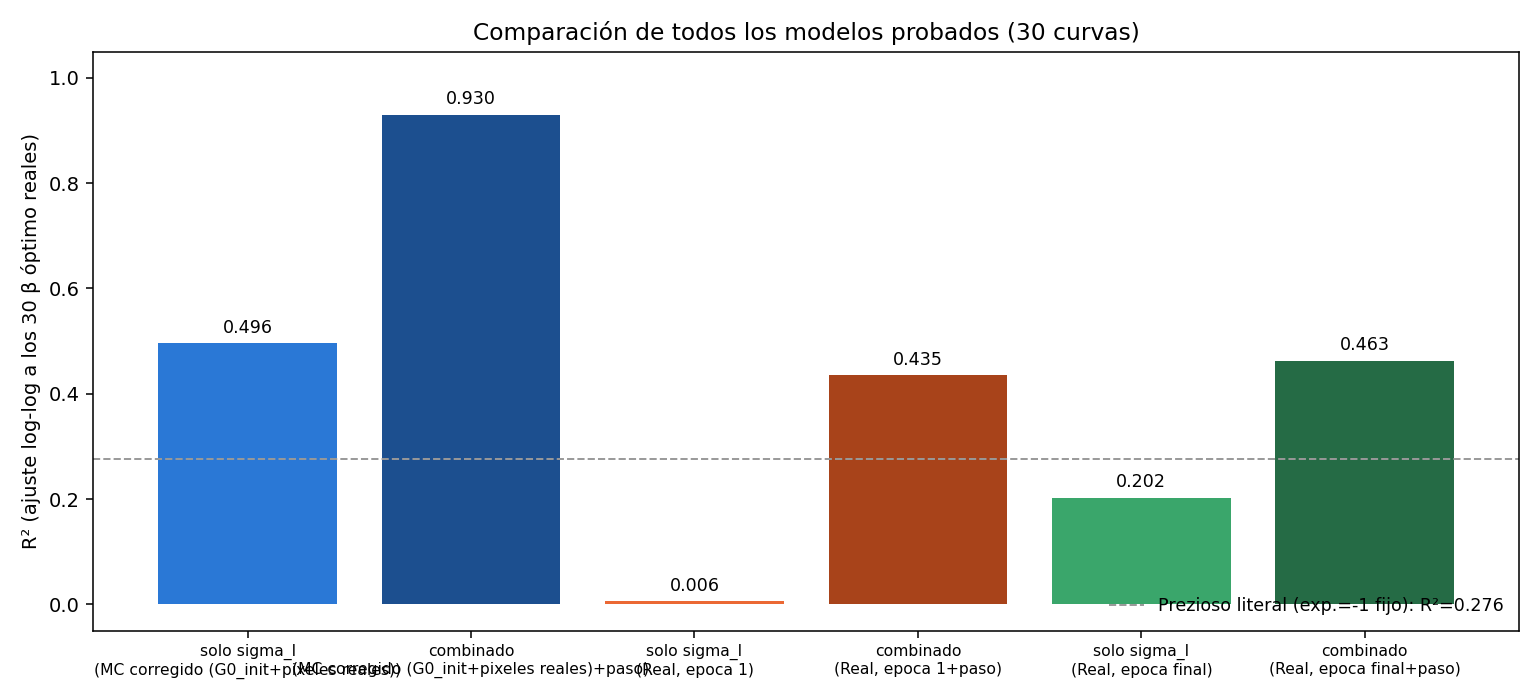
\includegraphics[width=.48\linewidth]{../reconstruccion_beta_optimo_30curvas/comparacion_R2_todos_los_modelos_30curvas.png}
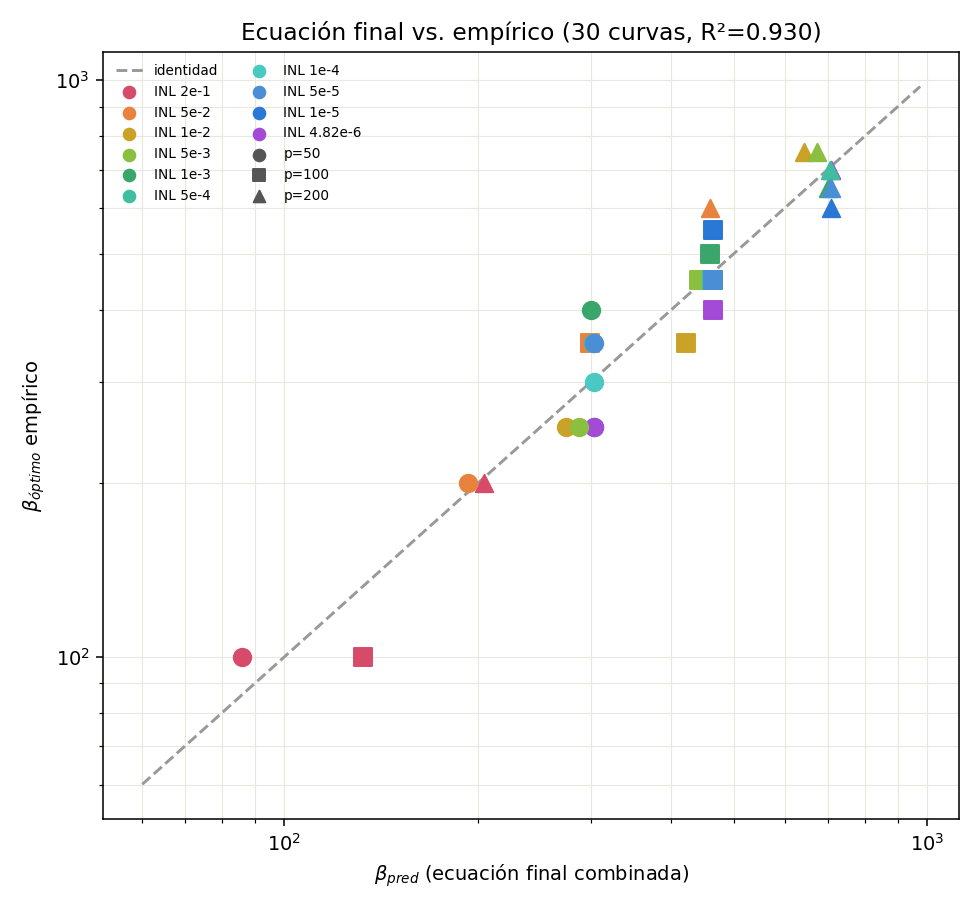
\includegraphics[width=.48\linewidth]{../reconstruccion_beta_optimo_30curvas/ecuacion_final_vs_empirico_30curvas.png}
\caption{Izq.: la forma literal de Prezioso/LeCun (exponente fijo en $-1$) da $R^2=0.276$;
dejar el exponente libre + paso\_medio da $R^2=0.930$. Der.: $\beta$ predicho vs. empírico,
30 curvas.}
\end{figure}

Más importante que el $R^2$: para cada una de las 30 curvas se buscó, en la \textbf{grilla
real de 40 $\beta$} ya corrida, el punto más cercano a la predicción de la fórmula, y se
comparó su accuracy contra el pico real de esa curva completa. \textbf{Las 30 de 30 curvas
alcanzan $\geq$99\,\% de su accuracy pico} (media 99.95\,\%, mínimo 99.38\,\%) usando la
$\beta$ predicha, sin ninguna búsqueda —a pesar de que el error puntual de la predicción llega
hasta $\pm$32\,\% en algunas curvas, porque el pico accuracy-vs-$\beta$ es ancho (meseta)
cerca del óptimo.

\begin{figure}[h]\centering
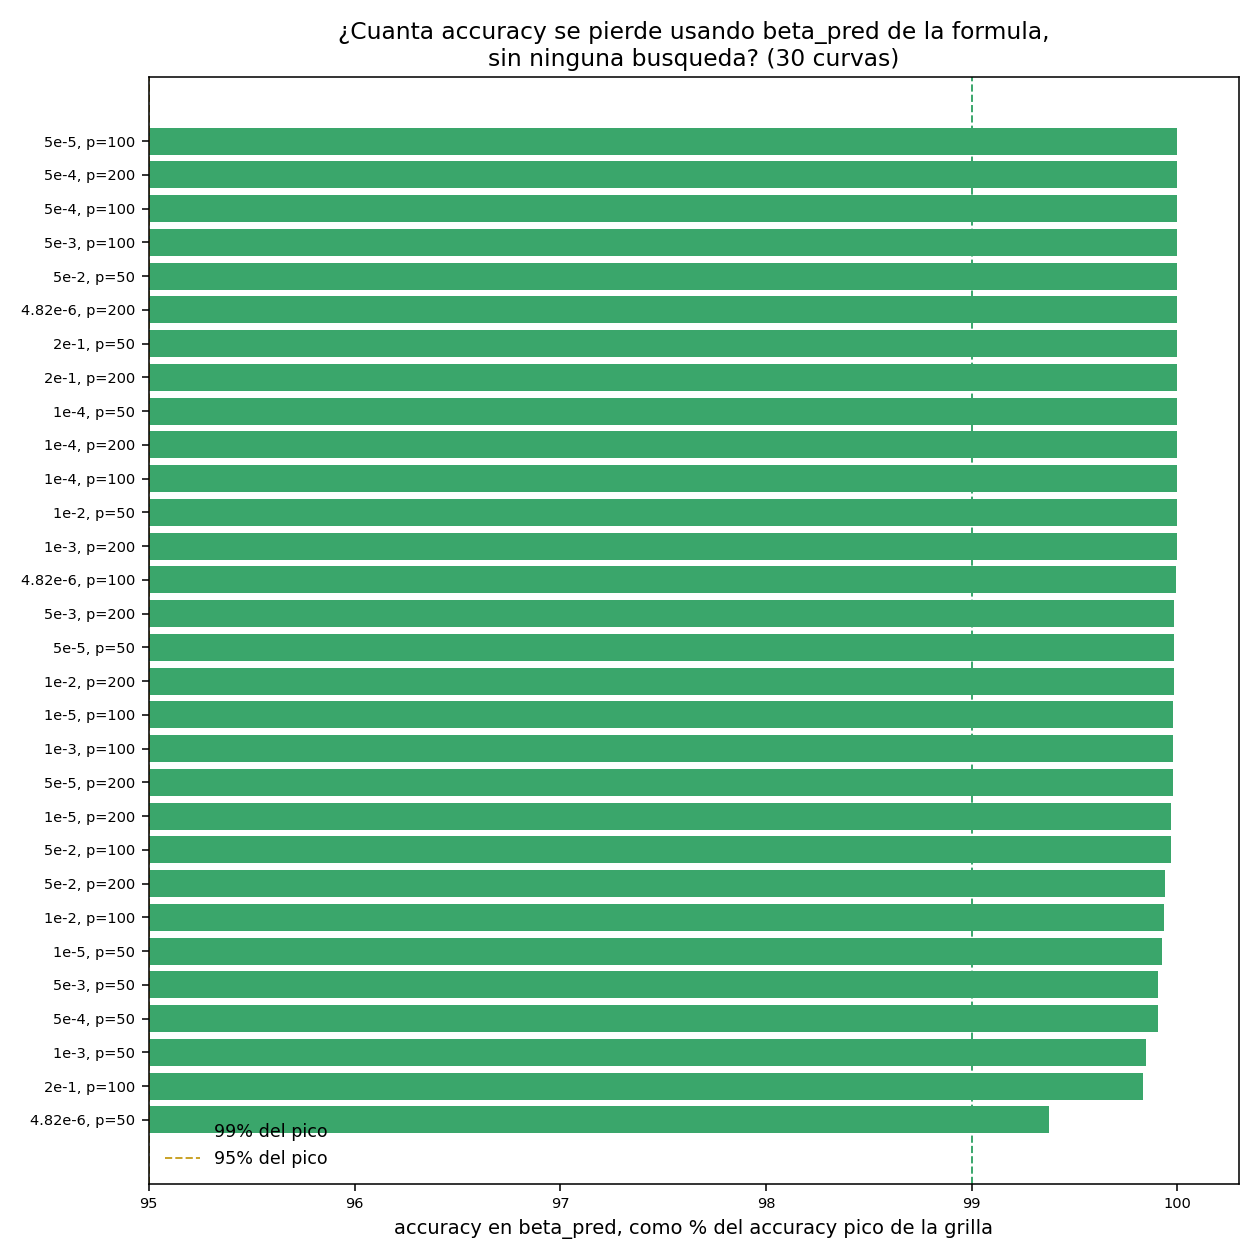
\includegraphics[width=.7\linewidth]{../reconstruccion_beta_optimo_30curvas/formula_vs_grilla_real.png}
\caption{$\beta$ predicho contra el punto de la grilla real de 40 $\beta$ más cercano, para las 30 curvas.}
\end{figure}

\section{Payoff práctico: una búsqueda mejorada}

\texttt{mejora\_search\_best\_beta/} usa este resultado para reemplazar la grilla ciega de
\texttt{search\_best\_beta()} (en producción: solo 2 puntos, $\beta\in\{1,300\}$) por una
grilla log-espaciada angosta, centrada en la predicción de la fórmula, con expansión
automática si el óptimo cae en el borde. Validación empírica (10 corridas por método, 2 combos
representativos, midiendo \emph{regret} real contra el ground truth de 100 épocas ya guardado):

\begin{table}[h]\centering
\begin{tabular}{lrrrr}\toprule
Método & regret medio & regret mediana & regret peor caso & tiempo \\\midrule
(a) original, como se usa hoy & 10.19 pp & 10.19 pp & 20.30 pp & 11.8 s \\
(b) original, defaults de fábrica & 0.24 pp & 0.03 pp & 2.16 pp & 118.2 s \\
\textbf{(c) mejorado} & \textbf{0.08 pp} & \textbf{0.04 pp} & \textbf{0.45 pp} & 218.2 s \\\bottomrule
\end{tabular}
\end{table}

El método (a) —el que corre hoy en \texttt{Crossbar\_train\_experimento\_beta\_por\_capa.py}—
elige $\beta=1$ en el combo más no lineal probado, perdiendo $\sim$20 puntos porcentuales de
accuracy frente al óptimo real. Validado además contra los 30 combos completos (no solo los 2
de la tabla): la fórmula predice el $\beta$ óptimo real dentro de un factor $1.26\times$ en el
peor de los 30 casos (mediana del cociente predicho/real: 0.948; 100\,\% de los casos dentro
de un factor $2\times$).

\section{Integración a producción}

Los pasos 3--7 documentan la fórmula validándose contra evidencia real, siempre como código
nuevo que importa la clase base sin tocarla (ver Sección 13). Una vez validada la mejora de la
Sección 7 como un parche aparte (subclase \texttt{MemDNNMejorado} en
\texttt{mejora\_search\_best\_beta/search\_best\_beta\_mejorado.py}), se integró directamente
en la clase base \texttt{MemDNN} (\texttt{MemCrossbarClass\_beta\_por\_capa.py}): un método
nuevo \texttt{search\_best\_beta\_mejorado()} con las mismas fórmulas y correcciones (common
random numbers, grilla log-espaciada centrada en \texttt{beta\_pred\_formula()}, meseta 1-SE),
y \texttt{Crossbar\_train\_experimento\_beta\_por\_capa.py} ya lo usa por defecto cuando
\texttt{optimize\_beta=True}, en vez del \texttt{search\_best\_beta()} original (que queda en
el archivo, sin uso por defecto). Es la \textbf{única} modificación al código base de todo
este hilo, y es posterior —y consecuencia directa— de la validación de las Secciones 4 a 7, no
una premisa de ellas.

\section{Chequeos de robustez adicionales}

Tres estudios adicionales pusieron a prueba los bordes del resultado anterior:
\texttt{validacion\_rango\_conductancia/} (sensibilidad al ratio $G_{max}/G_{min}$),
\texttt{mejora\_estimacion\_beta\_INL\_2e1\_a\_1e3/} (reestimación en la zona de transición de
INL) y \texttt{reconstruccion\_logits\_val\_INL\_1e-2\_p\_100\_beta1/} (sanity check: los
logits reconstruidos por Monte Carlo coinciden con los logits reales guardados del
entrenamiento). Ver el reporte de cada carpeta para el detalle.

\section{Síntesis cuantitativa del hilo completo}

\begin{table}[h]\centering
\begin{tabular}{lrlr}\toprule
Paso & $n$ curvas & Modelo & $R^2$ (log-log) \\\midrule
Validación fórmula analítica (solo $\sigma_W$) & 6 & $\beta=\kappa/\sigma_W$ & 0.678 \\
Fórmula propuesta ($\sigma_W$ + paso medio) & 6 & 2 factores & 0.947 \\
Reconstrucción, escala $3\times$ & 18 & 2 factores & 0.938 \\
Reconstrucción, escala $5\times$ & 30 & 2 factores & 0.930 \\\bottomrule
\end{tabular}
\caption{Los coeficientes del modelo de 2 factores casi no cambian entre 6, 18 y 30 curvas
—la señal más fuerte de que no es un sobreajuste a la muestra chica inicial.}
\end{table}

\section{Limitaciones honestas}

\begin{itemize}
\item \textbf{$N$ fijo.} Las 30 curvas comparten $N=784$ (fan-in de MNIST); el exponente
teórico de $N$ ($N^{-1/2}$) no se vuelve a poner a prueba con esta data.
\item \textbf{Un solo dataset.} Fashion-MNIST está disponible pero no se usó en este hilo.
\item \textbf{Ajuste in-sample.} Los $R^2$ se calculan sobre las mismas curvas usadas para
ajustar los coeficientes; la estabilidad de los coeficientes al escalar 6$\to$18$\to$30 es la
evidencia disponible en su lugar, no un reemplazo formal de un held-out set.
\item \textbf{Grilla de $\beta$ de 40 puntos, espaciados de a 50.} El $\beta$ óptimo empírico
contra el que se ajusta y valida tiene ese error de resolución incorporado.
\item \textbf{Solo $\beta$ global.} Ni la fórmula ni la búsqueda mejorada optimizan $\beta$
distinto por capa (hilo de trabajo separado, \texttt{exploracion\_beta\_capa\_oculta\_100/},
fuera del alcance de esta entrega).
\item \textbf{Errores puntuales de hasta $\pm$32\,\%} se traducen en pérdida de accuracy
despreciable ($\leq$1\,\%) porque el pico accuracy-vs-$\beta$ es ancho, pero eso no es lo
mismo que decir que la fórmula es precisa en $\beta$ —es precisa en el resultado práctico que
importa.
\end{itemize}

\section{Conclusión y recomendación}

La fórmula $\beta_{\text{óptimo}}\approx C\cdot\sigma_I^{-3}\cdot\mathrm{paso\_medio}^{-0.6}$
(constante y exponentes según la Sección 6) predice, sin entrenar nada, un $\beta$ que
alcanza $\geq$99\,\% del accuracy pico en las 30 configuraciones reales disponibles, y usada
para centrar \texttt{search\_best\_beta()} baja el regret medio de 10.19pp a 0.08pp con un
costo de cómputo despreciable frente a un entrenamiento completo. \textbf{Recomendación:}
usarla como pre-filtro barato antes de una búsqueda angosta de verificación —no como reemplazo
de la búsqueda en un solo paso sin verificar, dado que sigue siendo evidencia sobre un único
régimen (arquitectura SP, $N=784$, MNIST, ratio $G_{max}/G_{min}=10$).

\section{Registro de procedencia}

Cada carpeta del hilo (Secciones 3–7 y 9) tiene, en su propio reporte, una tabla
``registro de códigos usados'' con: qué script es nuevo, qué función se importó sin modificar
y de qué archivo, y qué dato de entrada se usó. Este reporte enlaza esas tablas en vez de
repetirlas. El código base (\texttt{MemCrossbarClass\_beta\_por\_capa.py},
\texttt{Crossbar\_train\_experimento\_beta\_por\_capa.py}) no fue modificado por ninguno de
esos reportes de validación —la única modificación es la integración a producción descripta
en la Sección 8, posterior a toda la validación. Mapa completo del repositorio, entorno y
cómo reproducir cada paso: ver \texttt{README.md} en la raíz del repositorio.

\bigskip
\noindent\textit{Generado a partir de reportes ya existentes y verificados de este mismo
proyecto; no se corrió ningún entrenamiento ni Monte Carlo nuevo para armar esta síntesis.}

\end{document}
